\documentclass{VUMIFPSbakalaurinis}
\usepackage{algorithmicx}
\usepackage{algorithm}
\usepackage{algpseudocode}
\usepackage{amsfonts}
\usepackage{amsmath}
\usepackage{bm}
\usepackage{caption}
\usepackage{color}
\usepackage{float}
\usepackage{graphicx}
\usepackage{listings}
\usepackage{subfig}
\usepackage{wrapfig}

\usepackage{enumitem}
\setitemize{noitemsep,topsep=0pt,parsep=0pt,partopsep=0pt}
\setenumerate{noitemsep,topsep=0pt,parsep=0pt,partopsep=0pt}

\hbadness=5000
% Titulinio aprašas
\university{Vilniaus universitetas}
\faculty{Matematikos ir informatikos fakultetas}
\department{Programų sistemų studijų programa}
\papertype{Mokslo tiriamasis darbas II}
\title{Srautinio apdorojimo sistemų balansavimas taikant mašininį mokymąsi}
\titleineng{Balancing stream processing systems using machine learning}
\author{Vytautas Žilinas}
\supervisor{Partn. doc. Andrius Adamonis}
\reviewer{Prof. dr. Aistis Raudys}
\date{Vilnius – \the\year}

% Nustatymai
% \setmainfont{Palemonas}   % Pakeisti teksto šriftą į Palemonas (turi būti įdiegtas sistemoje)
\bibliography{bibliografija}

\begin{document} 
\maketitle

\cleardoublepage\pagenumbering{arabic}
\setcounter{page}{2}

\section{Įvadas}

Šio darbo tikslas - apžvelgti susijusius literatūros šaltinius, pateikti jų santraukas ir panaudoti šią informacija suformuluoti problemą, kuri bus nagrinėjama sekančiame darbe. 

Realaus laiko duomenų apdorojimas (angl. real-time data processing) yra jau senai nagrinėjamas kaip vienas iš būdų apdoroti didelių kiekių duomenis (angl. Big data). Vienas iš realaus laiko apdorojimo sprendimų yra srautinis duomenų apdorojimas. Srautinis duomenų apdorojimas (angl. stream processing) – lygiagrečių programų kūrimo modelis, pasireiškiantis sintaksiškai sujungiant nuoseklius skaičiavimo komponentus srautais, kad kiekvienas komponentas galėtų skaičiuoti savarankiškai \cite{shortstreamproc}. 

Yra keli pagrindiniai srautinio apdorojimo varikliai: „Apache Storm“, „Apache Spark“, „Heron“ ir kiti. „Apache Storm“ ir „Heron“ apdoroja duomenis ne duomenų srautais, o „Apache Spark“ mikro-paketais \cite{karau2015learning}. „Heron“ srautinio apdorojimo variklis, buvo išleistas „Twitter“ įmonės 2016 metais kaip greitesnė alternatyva „Apache Storm“ srautinio apdorojimo varikliui \cite{openSourcing}.Šiame darbe bus naudojamas „Heron“, kadangi tai yra naujesnis ir greitesnis srautinio apdorojimo variklis nei „Apache Storm“ \cite{twitterHeron}. 

Srautinio apdorojimo sistemų balansavimas (angl. auto-tuning) - tai sistemos konfigūracijos valdymas siekiant užtikrinti geriausią resursų išnaudojimą - duomenų apdorojimas neprarandant greičio, bet ir naudojant tik reikiamą kiekį resursų. Kadangi srautinio apdorojimo sistemų komponentai yra kuriami kaip lygiagretus skaičiavimo elementai, todėl jie gali būti plečiami horizontaliai ir vertikaliai \cite{shortstreamproc} keičiant sistemų konfigūraciją. Tačiau lygiagrečių elementų kiekio keitimas nėra vienintelis būdas optimizuoti resursų išnaudojimą. Kiekvienas variklis turi savo rinkinį konfigūruojamų elementų. Darbe naudojamas „Heron“ variklis leidžia optimizuoti sistemas naudojant 56 konfigūruojamus svertus (angl. levers) \cite{configDocument}.

Yra skirtingi būdai kaip gali būti parenkama tinkama konfigūracija. Kadangi dar nėra naudojimui paruoštų sprendimų, kurie galėtų balansuoti srautinio apdorojimo sistemas savarankiškai, dažniausiai tai daro duomenų inžinieriai, kurie dirba su šiomis sistemomis. Kadangi srautinio apdorojimo sistemų apkrovos gali būti skirtingų pobūdžiu (duomenų kiekis, skaičiavimų sudėtingumas, nereguliari apkrova), o inžinieriai konfigūruodami išbando tik keletą derinių ir pasirenka labiausiai tinkanti \cite{selfRegulatingStreaming}, lieka labai daug skirtingų neišbandytų konfigūracijos variacijų. Optimalios konfigūracijos suradimas yra NP sudėtingumo problema \cite{automateTuning}, nes žmonėms yra sunku suvokti didelį kiekį konfigūracijos variacijų. 
Vienas iš būdų automatiškai valdyti konfigūraciją buvo pasiūlytas 2017 metų straipsnyje „Dhalion: self-regulating stream processing in heron“, kuriame autoriai aprašo savo sukurtą sprendimą „Dhalion“, kuris konfigūruoja „Heron“ srautinio apdorojimo sistemas pagal esama apkrova ir resursus, t.y. jei apdorojimo elementų išnaudojimas išauga >100\%, „Dhalion“ padidina lygiagrečiai dirbančių apdorojimo elementų kiekį \cite{dhalion}. Tačiau šis sprendimas leidžia reguliuoti tik elementų lygiagretumą ir tai daro tik reaktyviai.                         
Vienas iš naujausių būdų balansuoti srautinio apdorojimo sistemas - mašininis mokymasis. Vienas iš tokių bandymų buvo aprašytas 2018 metų straipsnyje „Auto-tuning Distributed Stream Processing Systems using Reinforcement Learning“, kuriame buvo atliktas tyrimas - „Apache Spark“ sistemos balansavimui buvo naudojamas skatinamojo mokymo REINFORCE algoritmas, kuris pagal dabartinę konfigūraciją ir gaunamas metrikas keitė srautinio apdorojimo sistemos konfigūracijas. Šiame tyrime buvo nustatyta, jog sprendimas, naudojantis mašininį mokymąsi, suranda konfigūraciją per trumpesnį laiką nei žmones ir taip pat sukurtą konfigūraciją naudojančios srautinio apdorojimo sistemos laukimo trukme (angl. latency) yra 60-70\% mažesnė nei tyrimo metu žmonių sukurtos konfigūracijos \cite{vaquero2018autotuning}. Šiame darbe naudojamas „Heron“ variklis leidžia prie savęs prijungti sukurtą išorinę metrikų surinkimo programą, kuri gali rinkti tokias sistemų metrikas kaip: naudojama RAM atmintis, CPU apkrova, komponentų paralelizmas ir kitas, kurios bus naudojamos sistemos balansavimui. 

Skatinamasis mokymasis yra vienas iš mašininio mokymosi tipų. Šis mokymasis skiriasi nuo kitų, nes nereikia turėti duomenų apmokymui, o programos mokosi darydamos bandymus ir klysdamos. Pagrindinis uždavinys naudojant skatinamąjį mokymąsi yra surasti balansą tarp naujų sprendimų tyrinėjimo (angl. exploration) ir turimos informacijos išnaudojimo (angl. exploitation) \cite{reinforcment}. Vienas iš pagrindinių privalumų naudojant skatinamąjį mokymąsi balansavimui - nereikia turėti išankstinių duomenų apmokymui kas leidžia jį paprasčiau pritaikyti skirtingoms srautinio apdorojimo sistemų apkrovoms. Tačiau tokio tipo mašininis mokymasis turi ir problemų: sudėtinga aprašyti tinkamos konfigūracijos apdovanojimo (angl. reward) funkciją ir turi būti teisingai aprašytas balansas tarp tyrinėjimo ir išnaudojimo tam, kad nebūtų patirti nuostoliai \cite{selfRegulatingStreaming}.

Yra sukurta daug skatinamojo mokymosi algoritmų (Monte Carl, Q-learning, Deep Q Network ir kiti), tad šiame darbe jie bus apžvelgti ir vienas iš jų bus pasirinktas ir pritaikytas išsikeltam uždaviniui. Algoritmas bus pasirinktas pagal tai, kuris yra tinkamiausias srautinių apdorojimų sistemų balansavimui.

\section{Srautinio apdorojimo sistemų matavimas ir derinimas}
\subsection{Srautinio apdorojimo sistemos}
Srautinis duomenų apdorojimas (angl. stream processing) – terminas naudojamas apibrėžti sistemas sudarytas iš skaičiavimo elementų (angl. modules) galinčių skaičiuoti lygiagrečiai ir kurios bendrauja kanalais. Tokios sistemų elementai dažniausiai skirstomi į tris klases: šaltinius (angl. sources) kurie paduoda duomenis į sistemą, filtrus (angl. filters) kurie atlieka tam tikrus vienetinius (angl. atomic) skaičiavimus ir nuotakus (angl. sink) kurie perduoda duomenis iš sistemų \cite{stephens1997survey}. 
\begin{figure}[H]
    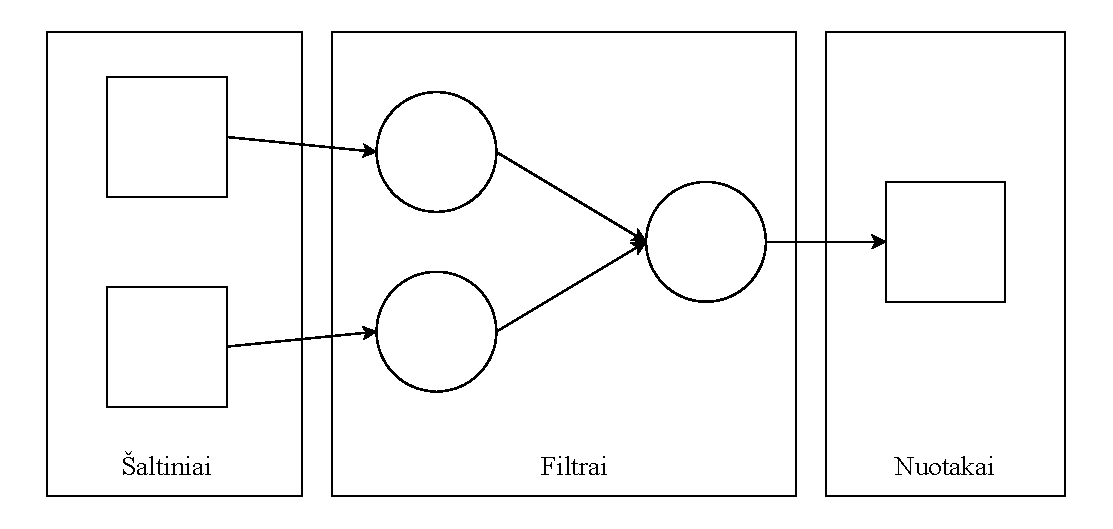
\includegraphics[width=15cm]{img/Srautinio apdorojimo sistema.pdf}
    \caption{Srautinio apdorojimo sistemos pavyzdys}
    \label{srautinio-apdorojimo-sistema}
\end{figure} 
Srautinio apdorojimo sistemos literatūroje yra vaizduojamos orientuotais grafikais (\ref{srautinio-apdorojimo-sistema} pav.). Srautinių apdorojimo sistemos skiriasi nuo reliacinių modelio \cite{babcock2002models}: 
\begin{itemize}
    \item Duomenys į sistemą patenka tinklu, o ne iš fizinių talpyklų.
    \item Duomenų patekimo tvarka negali būti kontroliuojama.
    \item Duomenų kiekis yra neapibrėžtas.
    \item Duomenys apdoroti srautinio apdorojimo sistema yra pašalinami arba archyvuojami, t.y. juos pasiekti yra sunku. 
\end{itemize}
\subsubsection{Duomenų vykdymas}
Srautinio apdorojimo sistemų veikimui reikalingas srautinio apdorojimo variklis (angl. stream processing engine). Šie varikliai yra skirti srautinio apdorojimo sistemų vykdymui, dislokavimui ir užtikrinti plečiamumą (angl. scaling) ir toleranciją gedimams (angl. fault-tolerance) \cite{zhao2017taxonomy}. Populiariųjų srautinio apdorojimo variklių pavyzdžiai: "Apache Storm", "Apache Heron, "Apache Spark", "Apache Samza" ir t.t \cite{roger2019comprehensive}. 
Duomenų vykdymas gali būti išskaidytas į tris komponentus \cite{zhao2017taxonomy}: 
\begin{itemize}
    \item Planavimas (angl. scheduling) - duomenų apdorojimo užduočių planavimas daro įtaką bendram srautinio apdorojimo veikimui \cite{falt2011task}. Pavyzdžiui "Apache Samza" naudoja "Apache YARN" resursų valdymo sistemą, kuri turi planavimo posistemę, kuri skirsto resursus \cite{noghabi2017samza} 
    \item Plečiamumas (angl. scalability) - apibrėžia daug apdorojimo branduolių turinčios sistemos gebėjimą apdoroti didėjanti kiekį užduočių ir galimybę didinti pačią sistemą kad susidoroti su didėjančių kiekiu duomenų \cite{bondi2000characteristics}. Srautinio apdorojimo varikliai turi užtikrinti srautinio apdorojimo sistemų plečiamumą \cite{stonebraker20058}.    
    \item Išskirstytas skaičiavimas (angl. Distributed computation) - tarpusavyje nesusiję skaičiavimo elementai turi naudotojam atrodyti kaip viena darni sistemą \cite{tanenbaum2007distributed}. Srautinio apdorojimo varikliai turi užtikrinti darbų paskirstymą ir skaičiavimo įrenginių koordinacija, kad daug duomenų būtų apdorojami vienu metu \cite{zhao2017taxonomy}.
\end{itemize}
Srautinio apdorojimo sistemos turi viena pagrindinį elementą - srauto procesorių (angl. stream processor), kuris apibrėžia sistemos elementus, aprašo kaip šie sistemos elementai sujungti ir pateikia nustatymus elementams \cite{zhao2017taxonomy}. Pavyzdžiui "Apache Storm" šis elementas vadinimas "topology", kuris yra užrašomas Java kalba naudojant "Apache Storm" pateiktą biblioteką \cite{iqbal2015big}.
\subsubsection{Duomenų priėmimas}
Į srautinio apdorojimo sistemą duomenis patenka per šaltinius, kurie šiuos duomenis perduoda tolimesniems elementams. Dažniausiai duomenis perduodami į sistemą naudojant žinučių eiles (angl. message queues), nes jos turi buferi, kas leidžia mažinti skirtumus tarp duomenų gavimo ir duomenų apdorojimo greičių, ir žinučių eilių brokeriai gali atfiltruoti duomenis ir nukreipti juos į tinkamus šaltinius \cite{kamburugamuve2016survey}. Tačiau šaltiniai turi turėti galimybę rinkti išsaugotus ir priimti ateinančius naujus duomenis \cite{stonebraker20058}, todėl nors ir šaltiniai dažniausiai priima srautinius duomenis, jie turi taip pat gebėti naudoti duomenis iš talpyklų \cite{zhao2017taxonomy}. 
\subsection{Srautinio apdorojimo sistemų matavimas}


\subsection{Srautinio apdorojimo sistemų derinimas}

\section{Srautinio apdorojimo sistemų duomenų pobūdis ir apkrovos}

\section{Skatinamojo mokymosi algoritmai}

\printbibliography[heading=bibintoc] 

\end{document}
